%%%%%%%%%%%%%%%%%%%%%%%%%%%%%%%%%%%%%%%%%%%%%%%%%%%%%%%%%%%%%%%%%%%%%%%
%%%%%%%%%%%%%%%%%%%%%%%%%%%%%%%%%%%%%%%%%%%%%%%%%%%%%%%%%%%%%%%%%%%%%%%
%%%%%                                                                 %
%%%%%     <file_name>.tex                                             %
%%%%%                                                                 %
%%%%% Author:      <author>                                           %
%%%%% Created:     <date>                                             %
%%%%% Description: <description>                                      %
%%%%%                                                                 %
%%%%%%%%%%%%%%%%%%%%%%%%%%%%%%%%%%%%%%%%%%%%%%%%%%%%%%%%%%%%%%%%%%%%%%%
%%%%%%%%%%%%%%%%%%%%%%%%%%%%%%%%%%%%%%%%%%%%%%%%%%%%%%%%%%%%%%%%%%%%%%%\\

In this section, we present our experimental results in order to validate our theoretical findings and prove the merits of the Heavy-Light architecture. First, we will use randomized task sets to compare an energy optimal partitioning to state-of-the-art heuristics with and without DTM. Afterwards, we will use fixed partitions to evaluate our DTM algorithms, with both synthetic and real-world benchmarks.

\noindent\textbf{Hardware Testbed:}
Since the Heavy-Light platform is not commercially available, we can only emulate heavy light behavior using a commercially available dual-core platform. In this work, we use the LPCXpresso54102 platform, which consists of a performance-oriented Cortex M4 core and an energy-efficient Cortex M0 core. 
The only difference with a Heavy-Light platform is that the LPC has heterogeneous microarchitectures. In order to emulate a Cortex M4-based Heavy-Light platform, we characterize our applications by running them on the M4 at different frequencies, recording their execution times and energy. To test our task allocation policies, the M0 is configured to consume either the same clock cycles or energy as a Light M4 core running a task at a given $F_{LC}$ would, depending on the experiment. Tasks are executed in bare metal and the communication between cores is minimal, so any overheads are negligible when compared to task execution lengths.

\begin{table}[!t]
	\centering
	\caption{Estimated Power Values for Heavy-Light Platform}
	\label{tab:power_numbers_exp}
	\begin{tabular}{|c|c|c|c|} \hline
		\textbf{Component} & $\mathbf{P_\mathrm{\mathbf{Active}}}$ & $\mathbf{P_\mathrm{\mathbf{Sleep}}}$ & $\mathbf{P_\mathrm{\mathbf{Difference}}}$\\ 
		\hline
		Heavy (100MHz)& 22.1 mW & 2 mW & 20.1 mW\\
		\hline
		Light (100MHz) & 15.5 mW & 1.4 mW & 14.1 mW\\ 
		\hline
		Light (80MHz) & 12.1 mW & 1.4 mW & 10.7 mW\\ 
		\hline
		Peripherals & 16.6 mW & 2 mW & 14.6 mW\\ 
		\hline
	\end{tabular}
\end{table}

%For emulation, the M4 is treated as HC and the M0 is treated as the LC. In the actual platform, both cores run at the same frequency of $100MHz$.
The makespan and power consumption of the platform is logged using a National Instruments USB-6216 Data Acquisition board. Table~\ref{tab:power_numbers_exp} shows the power consumption of the HC and LC at 100MHz. The former is the measured power consumption of the LPC's Cortex M4, and the ladder is the estimate of an M4 LC with reduced power density. The power consumption of the LC scales linearly with its operating frequency, $F_{LC}$.

The makespan improvement and energy savings from the Heavy-Light Platform are always compared to a Cortex M4 based, single-core platform. 
%Experimentally, the energy consumption of the HC is always measured. However, the energy consumption of the LC at different operating frequencies can only be estimated; since the LPC platform does not allow us to change the frequency of HC and LC cores independently. 
To allow a fair comparison, the energy consumption values for single-core were acquired by executing all the tasks on the HC and subtracting the energy consumed by the LC, which is kept in sleep state.

%Both cores can run at a maximum frequency of $100 MHz$. %We modified the software running on the M0 such that either the execution time or energy consumption of tasks, depending on what was being measured, would match that of an actual LC. This required a per-characterization step, during which the execution time and power consumption of tasks running on the HC, at both maximum and reduced frequencies, were recorded.

%We first study the performance of MLPT heuristic as a function of the number of randomly generated tasks. 
%As a first step, we conducted a simulation in Matlab in order to study the correlation between $\Delta$ and the total number of tasks partitioned to the two task bins.
We first compare the performance of DTM-E to a state-of-the-art heuristic called LP+BP. As was previously mentioned in Section~\ref{related}, the heuristic presented in \cite{Paterna} uses a Linear Programming (LP) formulation and a modified Bin Packing (BP) algorithm to reduce the energy consumption in accelerators. %\textbf{Add some additional lines here explaining LP+BP}.


 %In this algorithm, the total number of tasks and the sum of computation cycles can be set as parameters. Computation times of individual tasks are assigned randomly. In Figure~\ref{fig:delta-tasks}, we compare the performance of MLPT with an optimal task allocation policy; for different number of tasks and different values of $F_\mathrm{LC}$. As shown in Figure~\ref{fig:delta-tasks}, MLPT performs close to optimal for all simulations. Furthermore, $\Delta$ approaches $\Delta_\mathrm{opt}$ ($|{\Delta - \Delta_\mathrm{opt}}|_\mathrm{avg}\rightarrow 0$) for a reasonable number of randomly generated tasks ($\geq 10$). From this result, we can conclude that when the number of tasks $\geq 10$, MLPT approaches to the optimal task partition; which minimizes both makespan and energy consumption (Theorem~\ref{thm:delta_opt}).
%Later on, we conduct experiments assuming that $\Delta$ is fixed/given. We evaluate both synthetic benchmarks and a real-world application. 

%The task allocation was done by using the MLPT \cite{mlpt} heuristic, which is suitable for performance-constrained devices. Figure ~\ref{fig:delta-tasks} shows the results for different values of $F_\mathrm{LC}$. We note that even for a low number of tasks the divergence between $\Delta$ and $\Delta_\mathrm{opt}$ is not extensive. Furthermore, for $n \geq 10$ the convergence to $\Delta_\mathrm{opt}$ is almost absolute.\par
%\vspace{-1em}
%\begin{figure}[!hbtp]
%\centering
%  \includegraphics[width=0.8\columnwidth]{./figures/delta-tasks}
%  \caption{Correlation between $\Delta$ and the number of tasks}
%  \label{fig:delta-tasks}
%\end{figure}

\begin{figure}[!b]
	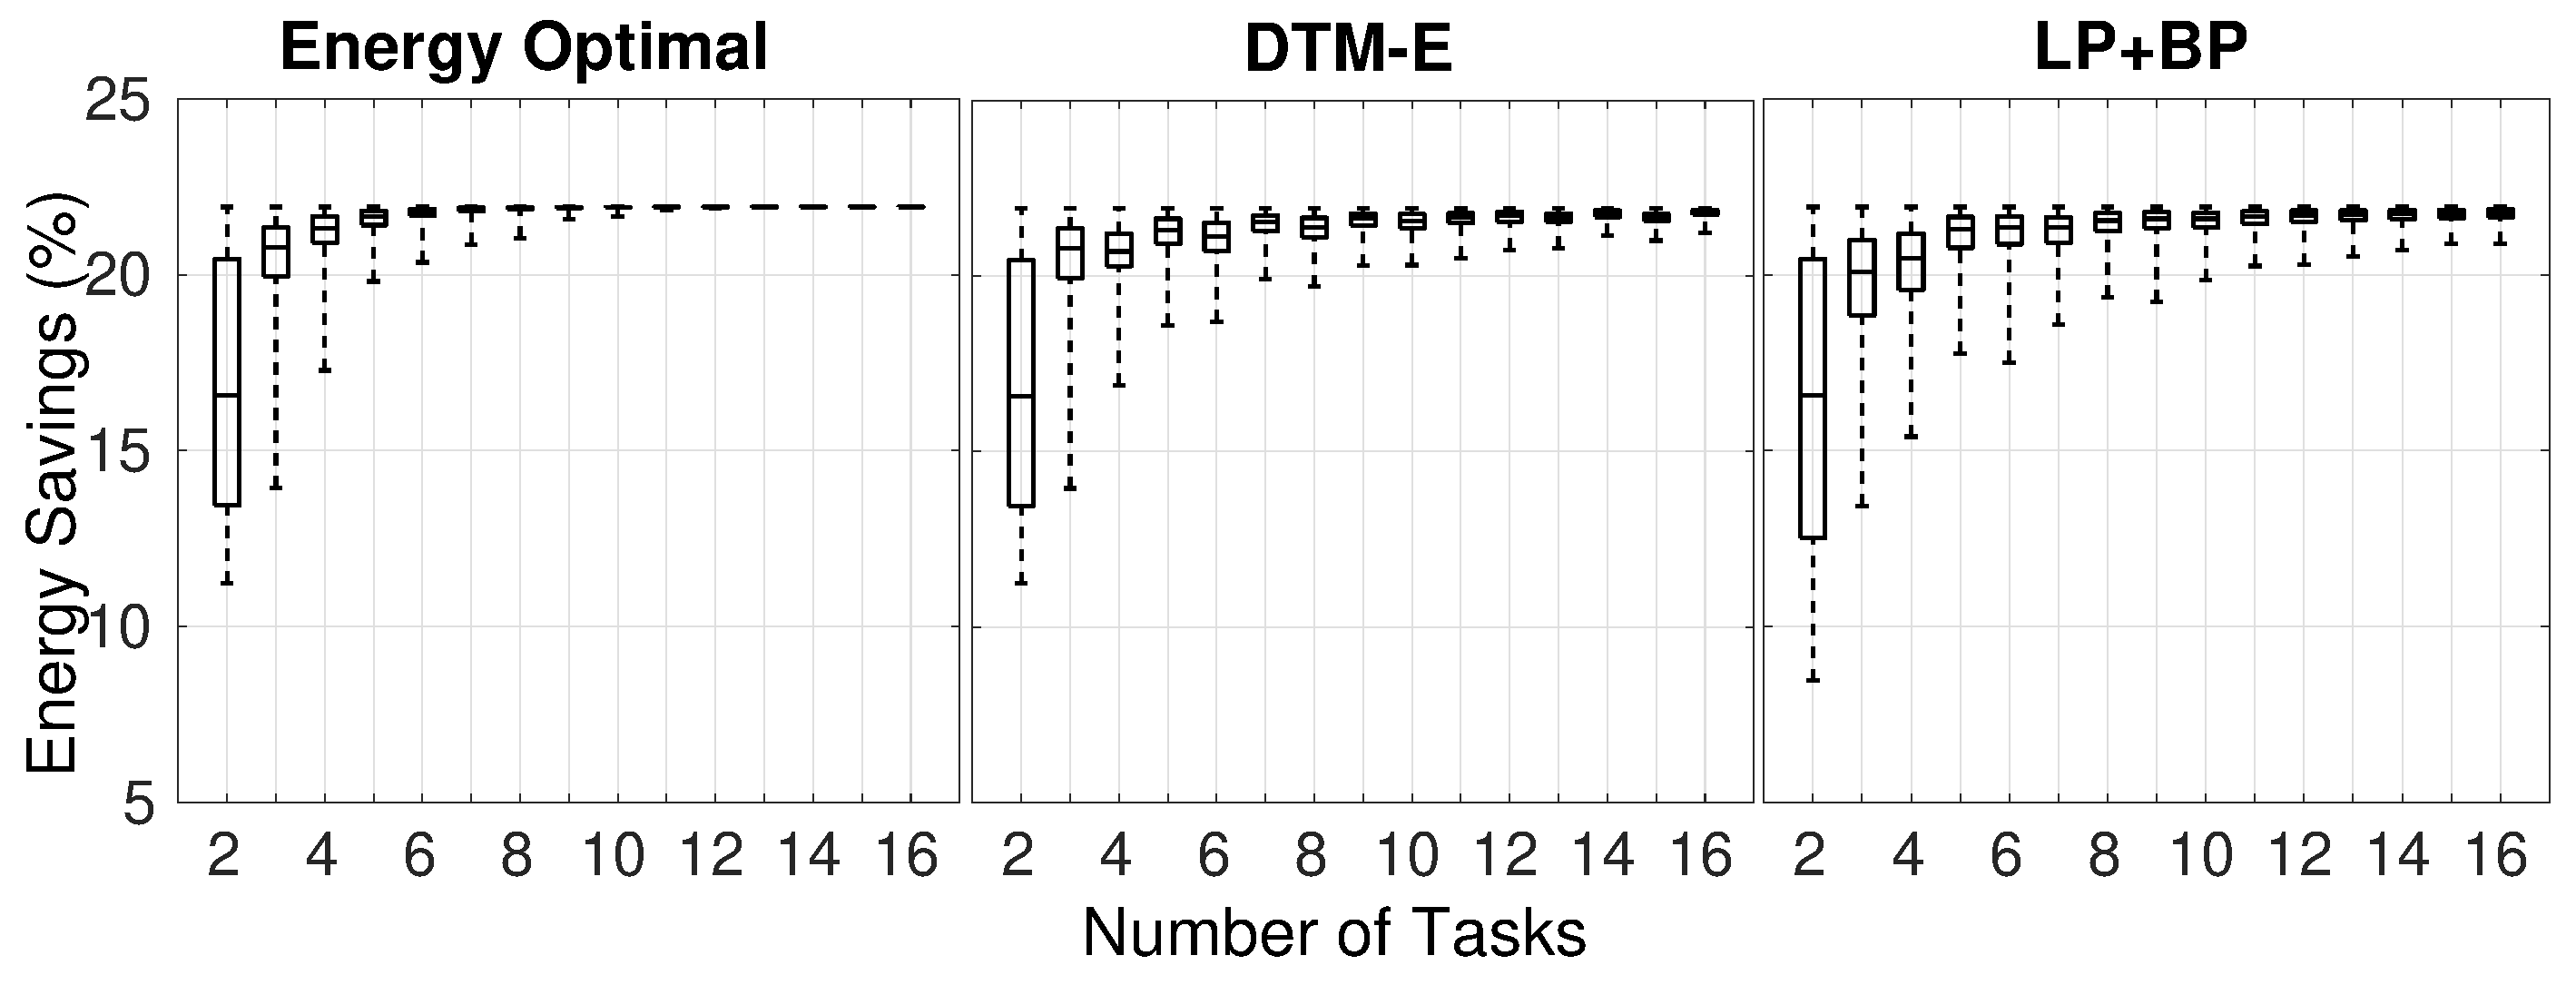
\includegraphics[width=\columnwidth]{./figures/opt_DTM_LPBP}
	\caption{Optimal vs DTM-E vs LP+BP}
	\label{fig:comparison}
\end{figure}

%\begin{figure}[!b]
%	\centering
%	\begin{subfigure}{.48\columnwidth}
%		\centering
%		\includegraphics[width=\columnwidth]{./figures/flc_80_delta_makespan_theory}
%		\caption{Makespan Simulation}
%		\label{fig:Flc80-delta-makespan-theory}
%	\end{subfigure}
%	\begin{subfigure}{.48\columnwidth}
%		\centering
%		\includegraphics[width=\columnwidth]{./figures/flc_80_delta_makespan}
%		\caption{Makespan Experiment}
%		\label{fig:Flc80-delta-makespan}
%	\end{subfigure}
%	\caption{Makespan Results for $F_{LC} = 80 MHz$ and utilization = 50\%.}
%	\label{fig:flow}
%\end{figure}

\noindent\textbf{Comparison with LP+BP and Optimal mapping:}

To compare DTM-E approach, we generated 150000 random task-sets with up to 16 tasks and 100\% utilization. \emph{UUniFast}\cite{uunifast} algorithm is used to synthetically generate tasksets with fixed number of tasks. During this comparison, we assumed that $F_{HC} = 100MHz$ and $F_{LC} = 80MHz$, and considered the power consumption of the components as shown in Table~\ref{tab:power_numbers_exp}. By applying both the optimal formulation, DTM-E scheme and the LP+BP algorithm, we estimated the energy savings compared to a single-core using Matlab. The results can be seen in Figure~\ref{fig:comparison}. Firstly, note that the performance of DTM-E is near optimal. The mean and second/third quartile values are nearly identical for all simulation points. However, the fourth quartile values are marginally different. %Notice that, when the number of tasks is low (2, 3, 4), there are some tasksets which have negative energy savings. This may seem in conflict with our theoretical results (Specifically Theorem~\ref{thm:parallel}). However, this is not a contradiction because the single-core power we compare against has no sleep power for the LC. Therefore, the sleep power dissipation of the single core is lower compared to the sleep power of the Heavy-Light platform. This inherent difference in system efficiency leads to some corner cases where energy consumption of the dual core is higher compared to the energy consumption of the single core. 
While all schemes converge towards 22\% energy savings as the number of tasks increase, there is a clear difference for a low number of tasks between LP+BP and Optimal/DTM-E. We notice that although the mean values of all three schemes are similar, for low number of tasks, the worst case for LP+BP (fourth quartile) is significantly lower compared to the worst-case for DTM-E and optimal results. The difference stems from the fact that applications targeted by LP+BP exhibit a high degree of parallelism. In other words, when $\Delta$ is close to $\Delta_\mathrm{opt}$. If two task bins have significantly different sizes (leading to a high $\Delta$), the LP+BP algorithm is expected to have lower energy savings.  
 

%We notice that the mean energy savings for tasksets having two tasks is 11.0062, 11.0062 and 10.687 for opt, DTM-E and LP+BP respectively. Furthermore, we also notice a difference in average values for tasksets having three tasks (16.6395 vs 16.6323 vs 16.1795). However, in general, the difference becomes less as the number of tasks increase. This is because the difference stems from the fact that applications targeted by LP+BP exhibit a high degree of parallelism. In other words, when $\Delta$ is close to $\Delta_\mathrm{opt}$. If two task bins have significantly different sizes (leading to a high $\Delta$), the LP+BP algorithm can have lower energy savings.  

%\vspace{-1em}
%\begin{figure}[!htb]
%	\centering
%	\begin{subfigure}{.48\columnwidth}
%		\centering
%		\includegraphics[width=\columnwidth]{./figures/energy_efficient}
%		\caption{DTM-E}
%		\label{fig:proposed_scheme}
%%%		\centering
%		\includegraphics[width=\columnwidth]{./figures/lpbp}
%		\caption{LP+BP Algorithm\cite{Paterna}}
%		\label{fig:lpbp}
%	\end{subfigure}
%	\vspace{-0.05in}
%	\caption{Energy Savings for randomly generated task sets.}
%	\label{fig:comparison}
%\end{figure}

\noindent\textbf{Evaluation using Synthetic Benchmarks: }
The synthetic benchmark evaluation is used to quantify the effects of the single-core utilization and $\Delta$ on performance/energy improvement. For each utilization-$\Delta$ pair, we run 100 iterations of the application on the hardware test-bed, logging both the makespan and energy consumption of the Heavy-Light and single-core architectures. During these experiments, we also assumed $F_{HC} = 100$MHz and $F_{LC} = 80$MHz.\par

\begin{figure}[!b]
\centering
\begin{subfigure}{.48\columnwidth}
  \centering
  \includegraphics[width=\columnwidth]{./figures/flc_80_util_makespan}
  \caption{Makespan Experiment}
  \label{fig:Flc80-util-makespan}
\end{subfigure}
\begin{subfigure}{.48\columnwidth}
  \centering
  \includegraphics[width=\columnwidth]{./figures/flc_80_util_energy}
  \caption{Energy Experiment}
  \label{fig:Flc80-util-energy}
\end{subfigure}
\vspace{-0.05in}
\caption{Makespan and Energy Savings for $F_{LC} = 80 MHz$.}
\label{fig:Flc80-util}
\end{figure}
%\vspace{-0.1in}

%\begin{figure}[!b]
%	\centering
%	\begin{subfigure}{.48\columnwidth}
%		\centering
%		\includegraphics[width=\columnwidth]{./figures/flc_80_delta_energy_theory}
%		\caption{Energy Simulation}
%		\label{fig:Flc80-delta-energy-theory}
%	\end{subfigure}
%	\begin{subfigure}{.48\columnwidth}
%		\centering
%		\includegraphics[width=\columnwidth]{./figures/flc_80_delta_energy}
%		\caption{Energy Experiment}
%		\label{fig:Flc80-delta-energy}
%	\end{subfigure}
%	\caption{Energy Savings for $F_{LC} = 80 MHz$ and utilization = 50\%.}
%	\label{fig:ins}
%\end{figure}	


\begin{figure*}[!tp]
	\centering
	\begin{subfigure}{.5\columnwidth}
		\centering
		\includegraphics[width=\columnwidth]{./figures/flow_makespan}
		\caption{Makespan Improvement}
		\label{fig:flow_makespan}
	\end{subfigure}
	\begin{subfigure}{.5\columnwidth}
		\centering
		\includegraphics[width=\columnwidth]{./figures/flow_energy}
		\caption{Energy Savings}
		\label{fig:flow_energy}
	\end{subfigure}
	\begin{subfigure}{.5\columnwidth}
		\centering
		\includegraphics[width=\columnwidth]{./figures/openshoe_makespan}
		\caption{Makespan-INS}
		\label{fig:openshoe_makespan}
	\end{subfigure}
	\begin{subfigure}{.5\columnwidth}
		\centering
		\includegraphics[width=\columnwidth]{./figures/openshoe_energy}
		\caption{Energy Savings-INS}
		\label{fig:openshoe_energy}
	\end{subfigure}
	\caption{Results for Pix4Flow and INS Benchmarks}
	\label{fig:Flc80-delta}
\end{figure*}

We first analyze the impact of single-core utilization on energy savings and makespan. In this set of experiments, we evaluate two values of $\Delta\in\{0.2, 0.5\}$. The results for this evaluation are presented in Figure~\ref{fig:Flc80-util}. In this case, the \% improvement in makespan remains constant as utilization is increased. Therefore, we plot the makespan improvement in the form of a bar graph in Figure~\ref{fig:Flc80-util-makespan}. %In the optimal case, the makespan is decreased by 44\% and the energy savings can reach up to 22\%. 
In general, the percentage improvement in energy consumption increases as the utilization increases. We have high energy savings when $\Delta = 0.2$, since it is close to $\Delta_\mathrm{opt}=\frac{100-80}{100+80}=0.11$. Furthermore, the two policies do not differ, as $\Delta \leq \Delta_\mathrm{diff}=0.37$. However, when $\Delta = 0.5$, the two policies differ and there is a tradeoff between performance and energy consumption. %Finally, it is important to mention that in both cases the Heavy-Light platform shows significant energy savings even for low utilization.\par

Now, we analyze the proposed schemes for different values of $\Delta$. Figure~\ref{fig:Flc80-delta} shows both theoretical results and experimental evaluation for utilization = 50\%. According to the plots, the optimal makespan improvement and energy savings are 44\% and 17\% respectively. Both $\Delta_\mathrm{opt}(\approx 0.11)$ and $\Delta_\mathrm{diff}(\approx 0.37)$ are in agreement with our theoretical findings. Though the amount of task-level parallelism, and consequently, the potential energy savings are highly application-dependent, we will show in the following section that different types of real-world applications can exhibit improvements in both energy and performance.
%Furthermore, as we illustrated in Figure~\ref{fig:delta-tasks}, a small number of tasks are required to coverage to the optimal value of $\Delta=\Delta_\mathrm{opt}$. Therefore, for majority of application scenarios, we will be operating close to $\Delta_\mathrm{opt}$, leading to high improvement in energy consumption and performance.

%By correlating Figures~\ref{fig:delta-tasks} and~\ref{fig:Flc80-delta} we can conclude that the combination of the Heavy-Light architecture and the MLPT heuristic can result into significant improvement both in performance and energy-consumption, even for a relatively low number of tasks. For example, for $F_{LC} = 80MHz$ and $n=5$ the makespan is reduced by 40\% and the energy consumption by 15\%. Even for $n=2$ the improvement in both metrics is non-negligible.\par

\noindent\textbf{Evaluation using Real-World Application:} In this evaluation, we demonstrate the impact of our policies on a real-world application. 
%We chose the Pix4Flow \cite{Pix4Flow} camera module, which serves as a reference for applications with high degree of task-level parallelism. This application corresponds to a workload with $\Delta = 0$ and utilization = 90\%. During these experiments, $F_{LC}$ is varied from $50MHz$ to $100MHz$ in steps of $10MHz$.
We consider two different embedded applications: 1) Pix4Flow \cite{Pix4Flow} camera module, 2) open-source Inertial Navigation System (INS)~\cite{INS}. Pix4Flow has high task level parallelism while INS has low task-level parallelism. Though the INS benchmark has dependencies between some tasks, we ignore them to determine the partitioning and respect them when executing the application. During these experiments, $F_{LC}$ is varied from $50MHz$ to $100MHz$ in steps of $10MHz$. %\textbf{(TODO: State $\Delta$s for these applications)} \par

As shown in Figures~\ref{fig:flow_makespan} and~\ref{fig:flow_energy}, in the case of the Pix4Flow benchmark, the differences between the two task allocation policies are very narrow. This is due to the high degree of task-level parallelism in this application. Interestingly, even in the pessimistic case of $F_{LC} = 50MHz$, both  policies offer approximately 4\% energy savings. Both makespan improvement and energy savings increase proportionally to $F_{LC}$ and can reach up to 50\% and 22\% respectively. %\par

%However, as shown in Figures~\ref{fig:openshoe_makespan} and~\ref{fig:openshoe_energy}, the two allocation policies show very different behavior in the case of the INS benchmark. The performance-oriented policy offers a constant makespan improvement of approximately 14\% and , due to the low task-level parallelism. 
%On the other hand, the allocation of tasks is not always the same in the case of the energy-efficient policy. As you can see in Figure~\ref{fig:openshoe_makespan}, for $F_{LC} = 80MHz$, the makespan starts increasing, until it reaches its maximum value again for $F_{LC} = 100MHz$. Moreover, the energy savings are also limited, reaching up to only 5\%. 

For the INS application, the two allocation policies show a very different behavior. This is shown in Figures~\ref{fig:openshoe_makespan} and~\ref{fig:openshoe_energy}. The difference is due to the low task-level parallelism present in the application. When $F_{LC} \geq 80MHz$, the two policies start differing. The energy-efficient policy shows a small improvement in energy consumption (up to 5\%). However, the improvement in energy comes at the cost of loss in performance; with makespan degradation of up to 8\% compared to single-core due to the LC executing the bigger task bin. The performance-oriented policy has a constant makespan improvement of approximately 14\% with a slight increase in energy consumption, since the larger task bin is always executed by the HC. %This result shows that our DTM algorithms can still be applied to dependent task-sets and obtain energy savings. %As mentioned earlier,  



%\begin{figure}[!btp]
%	\centering
%	\begin{subfigure}{.48\columnwidth}
%		\centering
%		\includegraphics[width=\columnwidth]{./figures/flow_makespan}
%		\caption{Makespan Improvement}
%		\label{fig:flow_makespan}
%	\end{subfigure}
%	\begin{subfigure}{.48\columnwidth}
%		\centering
%		\includegraphics[width=\columnwidth]{./figures/flow_energy}
%		\caption{Energy Savings}
%		\label{fig:flow_energy}
%	\end{subfigure}
%	\caption{Results for Pix4Flow Benchmark}
%	\label{fig:flow}
%\end{figure}
%
%\begin{figure}[!btp]
%	\centering
%	\begin{subfigure}{.48\columnwidth}
%		\centering
%		\includegraphics[width=\columnwidth]{./figures/openshoe_makespan}
%		\caption{Makespan-INS}
%		\label{fig:openshoe_makespan}
%	\end{subfigure}
%	\begin{subfigure}{.48\columnwidth}
%		\centering
%		\includegraphics[width=\columnwidth]{./figures/openshoe_energy}
%		\caption{Energy Savings-INS}
%		\label{fig:openshoe_energy}
%	\end{subfigure}
%	\caption{Results for INS Benchmark}
%	\label{fig:ins}
%\end{figure}	

